\subsection{逐差法求加速度}
我们首先说明为什么要用逐差法来处理问题,因为实验有误差,我们处理的原则是让误差尽可能小.一般毫米刻度尺的绝对误差是$1mm$,如图\ref{fig:rulemm}所示
\begin{figure}[H]
  \centering
  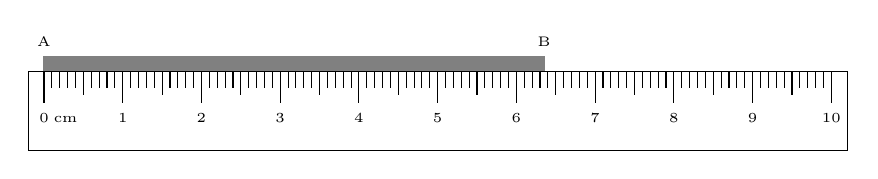
\begin{tikzpicture}
    \foreach \x in {
      0.1,0.2,0.3,0.4,0.6,0.7,0.8,0.9,
      1.1,1.2,1.3,1.4,1.6,1.7,1.8,1.9,
      2.1,2.2,2.3,2.4,2.6,2.7,2.8,2.9,
      3.1,3.2,3.3,3.4,3.6,3.7,3.8,3.9,
      4.1,4.2,4.3,4.4,4.6,4.7,4.8,4.9,
      5.1,5.2,5.3,5.4,5.6,5.7,5.8,5.9,
      6.1,6.2,6.3,6.4,6.6,6.7,6.8,6.9,
      7.1,7.2,7.3,7.4,7.6,7.7,7.8,7.9,
      8.1,8.2,8.3,8.4,8.6,8.7,8.8,8.9,
      9.1,9.2,9.3,9.4,9.6,9.7,9.8,9.9,
    }
    \draw (\x,0)--(\x,-0.2);
    \foreach \y in {0,1,2,3,4,5,6,7,8,9,10}
    \draw (\y,0)--(\y,-0.4) node [anchor=north]{\tiny \y};
    \foreach \z in {0.5,1.5,2.5,3.5,4.5,5.5,6.5,7.5,8.5,9.5}
    \draw (\z,0)--(\z,-0.3);
    \draw (-0.2,0) rectangle (10.2,-1);
    \draw (0,-0.6) node [anchor=west]{\tiny cm};
    \filldraw [color=gray] (0,0.02) rectangle (6.35,0.2);
    \draw (0,0.2) node [anchor=south]{\tiny A};
    \draw (6.35,0.2) node [anchor=south]{\tiny B};
  \end{tikzpicture}
  \caption{毫米刻度尺绝对误差}
  \label{fig:rulemm}
\end{figure}

在图\ref{fig:rulemm}中,测量一个杆的长度,使$A$ 端与零刻度线对齐,然后读$B$ 端的读数就是杆的长度.但是$B$不是完全与某一个刻度线对齐的,仔细观察不难发现它是一个介于$6.3mm$ 和$6.4mm$的数,所以坐标$x_B$ 的读数误差最大也就是$6.4mm-6.3mm=1mm$.对于一条纸带,我们在测量距离时,如图\ref{fig:zhidai}所示

\begin{figure}[H]
  \centering
  \begin{tikzpicture}
    \foreach \x in {
      0.1,0.2,0.3,0.4,0.6,0.7,0.8,0.9,
      1.1,1.2,1.3,1.4,1.6,1.7,1.8,1.9,
      2.1,2.2,2.3,2.4,2.6,2.7,2.8,2.9,
      3.1,3.2,3.3,3.4,3.6,3.7,3.8,3.9,
      4.1,4.2,4.3,4.4,4.6,4.7,4.8,4.9,
      5.1,5.2,5.3,5.4,5.6,5.7,5.8,5.9,
      6.1,6.2,6.3,6.4,6.6,6.7,6.8,6.9,
      7.1,7.2,7.3,7.4,7.6,7.7,7.8,7.9,
      8.1,8.2,8.3,8.4,8.6,8.7,8.8,8.9,
      9.1,9.2,9.3,9.4,9.6,9.7,9.8,9.9,
    }
    \draw (\x,0)--(\x,-0.2);
    \foreach \y in {0,1,2,3,4,5,6,7,8,9,10}
    \draw (\y,0)--(\y,-0.4) node [anchor=north]{\tiny \y};
    \foreach \z in {0.5,1.5,2.5,3.5,4.5,5.5,6.5,7.5,8.5,9.5}
    \draw (\z,0)--(\z,-0.3);
    \draw (-0.2,0) rectangle (10.2,-1);
    \draw (0,-0.6) node [anchor=west]{\tiny cm};
    \draw (-0.2,-0.4)--(-0.4,-0.4)--(-0.4,0.5)--(10.4,0.5)--(10.4,-0.4)--(10.2,-0.4);
    \foreach \x in {0,0.2,0.8,1.8,3.2,5,7.2,9.8}
    \filldraw [color=black] (\x , 0.05) circle [radius=1pt];
    \foreach \x in {0,0.2,0.8,1.8,3.2,5,7.2,9.8}
    \draw (\x , 0.05) node [anchor=south] {\tiny \thepointnum\stepcounter{pointnum}};
  \end{tikzpicture}
  \caption{测量纸带上点的距离}
  \label{fig:zhidai}
\end{figure}

在图\ref{fig:zhidai}中,使纸带上的计数点$0$ 与刻度尺上的零刻度对齐,然后依次读取其它点的读数,这些读数记作$x_i' \quad (i=0,1,2 \cdots)$,在纸带上标出这些读数如\ref{fig:zhidaidushu}所示

\setcounter{pointnum}{0}
\begin{figure}[H]
  \centering
  \begin{tikzpicture}
    \draw (-0.4,-0.4) rectangle (10.4,0.5); 
    \foreach \x in {0,0.2,0.8,1.8,3.2,5,7.2,9.8}
    \filldraw [color=black] (\x , 0.05) circle [radius=1pt];
    \foreach \x in {0,0.2,0.8,1.8,3.2,5,7.2,9.8}
    \draw (\x , 0.05) node [anchor=south] {\tiny \thepointnum\stepcounter{pointnum}};
    \draw (0,0)--(0,-0.8);
    \draw (0.2,0)--(0.2,-0.15);
    \draw [->,>=stealth] (0,-0.1)--(0.2,-0.1) ;
    \draw (0.2,-0.15) node {\tiny $x_1'$};
    \draw (0.8,0)--(0.8,-0.25);
    \draw [->,>=stealth] (0,-0.2)--(0.8,-0.2); 
    \draw (0.8,-0.3) node [anchor=south east] {\tiny $x_2'$};
    \draw (1.8,0)--(1.8,-0.35);
    \draw [->,>=stealth] (0,-0.3)--(1.8,-0.3) node [anchor=south east] {\tiny $x_3'$};
    \draw (3.2,0)--(3.2,-0.45);
    \draw [->,>=stealth] (0,-0.4)--(3.2,-0.4)node [anchor=south east] {\tiny $x_4'$};
    \draw (5,0)--(5,-0.55);
    \draw [->,>=stealth] (0,-0.5)--(5,-0.5)node [anchor=south east] {\tiny $x_5'$};
    \draw (7.2,0)--(7.2,-0.65);
    \draw [->,>=stealth] (0,-0.6)--(7.2,-0.6)node [anchor=south east] {\tiny $x_6'$};
    \draw (9.8,0)--(9.8,-0.75);
    \draw [->,>=stealth] (0,-0.7)--(9.8,-0.7)node [anchor=south east] {\tiny $x_7'$};
  \end{tikzpicture}
  \caption{计数点的读数标记}
  \label{fig:zhidaidushu}
\end{figure}

我们以不带撇号的坐标表示两点间的距离,如图\ref{fig:zhidaijvli}所示

\setcounter{pointnum}{0}
\begin{figure}[H]
  \centering
  \begin{tikzpicture}
    \draw (-0.4,-0.4) rectangle (10.4,0.5); 
    \foreach \x in {0,0.2,0.8,1.8,3.2,5,7.2,9.8}
    \filldraw [color=black] (\x , 0.05) circle [radius=1pt];
    \foreach \x in {0,0.2,0.8,1.8,3.2,5,7.2,9.8}
    \draw (\x , 0.05) node [anchor=south] {\tiny \thepointnum\stepcounter{pointnum}};
    \draw [<-,>=stealth] (0.2,0.05)--(0.4,0.05);
    \draw (0.5,0.05) node {\tiny $x_2$};
    \draw [->,>=stealth] (0.6,0.05)--(0.8,0.05);
    \draw [<-,>=stealth] (0.8,0.05)--(1.15,0.05);
    \draw (1.3,0.05) node {\tiny $x_3$};
    \draw [->,>=stealth] (1.45,0.05)--(1.8,0.05);
    \draw [<-,>=stealth] (1.8,0.05)--(2.35,0.05);
    \draw (2.5,0.05) node {\tiny $x_4$};
    \draw [->,>=stealth] (2.65,0.05)--(3.2,0.05);
    \draw [<-,>=stealth] (3.2,0.05)--(3.95,0.05);
    \draw (4.1,0.05) node {\tiny $x_5$};
    \draw [->,>=stealth] (4.25,0.05)--(5,0.05);
    \draw [<-,>=stealth] (5,0.05)--(5.95,0.05);
    \draw (6.1,0.05) node {\tiny $x_6$};
    \draw [->,>=stealth] (6.25,0.05)--(7.2,0.05);
    \draw [<-,>=stealth] (7.2,0.05)--(8.35,0.05);
    \draw (8.5,0.05) node {\tiny $x_7$};
    \draw [->,>=stealth] (8.65,0.05)--(9.8,0.05);
  \end{tikzpicture}
  \caption{计数点的距离标记}
  \label{fig:zhidaijvli}
\end{figure}

由于我在这里作图是按照标准的$1:3:5:7:9:11$ 完成的,第一段的距离太小,为了防止第一段看不清楚,所以在第一段上没有标出$x_1$,同时由图 \ref{fig:zhidaidushu}和图\ref{fig:zhidaijvli}对比可知两种表示方法的关系为

\begin{equation}
  x_i=x_i'-x_{i-1}' \qquad (i=1,2,3 \cdots)
  \label{eq:dushujvli}
\end{equation}

下面我们讨论加速度的计算,由$x_2$ 和$x_1$ 我们可以计算加速度,如下
\begin{gather}
  x_2-x_1=a_1T^2
  \intertext{经过简单计算可得}
  a_1=\frac{x_2-x_1}{T^2}
  \intertext{同理也可以得到加速度}
  a_2=\frac{x_3-x_2}{T^2}\\
  a_3=\frac{x_4-x_3}{T^2}\\
  a_4=\frac{x_5-x_4}{T^2}
  \intertext{由于在$a_1$的分子部分需要三个坐标来确定这个差,所以它的误差为$3mm$,$a_2$和$a_3$需要四个坐标来确定分子部分的差,所以其误差为$4mm$,但$T$是相同的,下面我们将这四个加速度取几何平均,则得到}
  a_{1234}=\frac{1}{4}(a_1+a_2+a_3+a_4)=\frac{x_5-x_1}{4T^2}
  \intertext{上面这个平均加速度,其分子部分需要三个坐标确定,但是分子上需要除以$4$,所以它的误差为$3mm/4=0.75mm$,同理我们可以得到$a_{2345}$等类似的平均值,如下}
  a_{2345}=\frac{1}{4}(a_2+a_3+a_4+a_5)=\frac{x_6-x_2}{4T^2}\\
  a_{3456}=\frac{1}{4}(a_3+a_4+a_5+a_6)=\frac{x_7-x_3}{4T^2}
  \intertext{上面的$a_{2345}$和$a_{3456}$的分子部分需要4个坐标确定,所以它们的误差是$4mm/4=1mm$,但是如果再取一次平均,如下}
  a=\frac{1}{3}(a_{1234}+a_{2345}+a_{3456})=\frac{(x_5+x_6+x_7)-(x_1+x_2+x_3)}{3\times 4T^2}
  \intertext{上式分子部分等于$x_7'-x_4'-x_3'$,用到了三个读数,但是分母上需要除以$12$ 所以它的误差是$3mm/12=0.25mm$,所以最后这个结果误差是最小的,为我们所采纳,这就是逐差法公式.下面我们总结写出加速度的方法,分母上的这个数值可以这样来确定:分子中的括号中有$3$个数值,同时每个数值的下标差相同(比如$5-1=4$,$6-2=4$,$7-3=4$),分母上的这个数值就是$3\times4=12$,同理我们可以写出$6$段和$9$段的计算公式如下}
  a=\frac{(x_4+x_5+x_6)-(x_1+x_2+x_3)}{3\times3 T^2}\\
  a=\frac{(x_6+x_7+x_8+x_9)-(x_1+x_2+x_3+x_4)}{4\times5 T^2}
  \intertext{有许多人为了方便记住逐差法的公式,在偶数段时将纸带一分为二,比如$6$段时,可以写作}
  a=\frac{(x_4+x_5+x_6)-(x_1+x_2+x_3)}{(3T)^2}
  \intertext{这可以理解为时间间隔为$3T$ 的两大段,使用$\Delta x=aT^2$ 一步写出,但是在遇到奇数段(比如$7$段)的时候就会遇到麻烦,如果按这个逻辑,可以选用前$6$段或者后$6$段,这样写出的公式误差是$3mm/9=0.33mm$,而按逐差法写出的公式是\CJKunderwave{去掉中间一段}这样计算的结果误差为$3mm/12=0.25mm$,显然\CJKunderwave{去掉中间一段}才能得到更精确的答案.}
  \notag
\end{gather}
\subsection{习题精解二}
\begin{calculate}
11.一滴雨滴从离地面 $20m$ 高的楼房屋檐自由下落,下落过程中用 $0.2s$ 的时间通过一个窗口,窗口的高度为 $2m$ , $g$ 取 $10m/s^2$ ,问:
[1]雨滴落地时的速度大小;
[2]雨滴落地前最后 $1s$ 内的位移大小;
[3]屋檐离地面的上边框有多高?

a.见解析

e.(1)由匀变速直线运动速度与位移的关系可得
$$v^2=2gh \Longrightarrow v=\sqrt{2gh}=20m/s$$

ee.(2)法一:雨滴在最后$1s$内的平均速度等于中间时刻的瞬时速度,中间时刻到最后共经历 $t_1=0.5s$ 所以有
$$v=\overline{v}+gt_1 \Longrightarrow \overline{v}=v-gt_1=15m/s$$
由位移等于平均速度乘以时间得
$$\Delta h=\overline{v}\Delta t_1 =15m$$

ee.法二:仍然采用平均速度的方法,先求出总时间,然后再求出最后$1s$的中间时刻,即
$$h=\frac{1}{2}gt^2 \Longrightarrow t=\sqrt{\frac{2h}{g}}=2s$$
所以最后$1s$ 的中间时刻即 $t=1.5s$ 时瞬时速度等于平均速度
$$\overline{v}=gt=15m/s$$
由位移等于平均速度乘以时间得
$$\Delta h=\overline{v}\Delta t_1 =15m$$

ee.法三:先求出总时间,然后再算出前 $1s$ 的时刻,并求出位移和总位移作差也可以得到最后 $1s$ 内的位移.即
$$h=\frac{1}{2}gt^2 \Longrightarrow t=\sqrt{\frac{2h}{g}}=2s$$
从下落开始到落地前$1s$经历的时间为$t_1=1s$ ,所以
$$h_1=\frac{1}{2}gt_1^2=5m$$
最后$1s$ 内的位移为
$$\Delta h=h-h_1=20m-5m=15m$$


ee.(3)在雨滴通过窗口的过程中,用时$0.2s$,所以它的中间时刻的瞬时速度等于平均速度为
$$\overline{v'}=\frac{2m}{0.2s}=10m/s$$
所以雨滴由屋檐到通过窗口的中间时刻所用时间为
$$t_0=\frac{\overline{v'}}{g}=1s$$
由此可得,雨滴由屋檐到窗口的时间为$t'=1s-0.1s=0.9s$ 所以屋檐离窗口上边框的高度为
$$h'=\frac{1}{2}gt'^2=4.05m$$

12.一辆值勤的警车停在公路边,当警员发现从他旁边以$10m/s$ 的速度匀速行驶的货车严重超载时,决定前去追赶,经过$5.5s$ 后警车发动起来,并以$2.5m/s^2$的加速度做匀加速运动,但警车的行驶速度必须控制在$90km/h$以内,问:
[1]警车在追赶货车的过程中,两车的最大距离是多少?
[2]警车发动后要经过多长时间 才能追上货车?

a.(1) 75m \qquad (2) 12s

e.(1)以警车发动起来作为计时起点,首先将警车的最大速度切换成国际单位 $90km/h=25m/s$ ,则警车的加速过程的持续时间$t_m$ 为
$$v_m=at_m \Longrightarrow t_m=\frac{v_m}{a}=10s$$
写出$0\sim 10s$ 内两车的距离为
$$\Delta x=55+10t -\frac{5}{4}t^2$$
整理成标准一元二次方程
$$\Delta x =-\frac{5}{4}t^2+10t+55 \quad (m)$$
由二次函数的知识,易得在$0\sim 10s$内 $t=4s$ 时距离最大,为
$$\Delta x_{max}=75m$$

ee.注意,在警车追赶货车的过程中,要分两步考虑,在$0\sim 10s$ 内,两车的距离关系才是上述的一元二次函数,但是这个过程不一定就追上,所以不能直接使用$\Delta x=0$ 来计算出时间,这就导致错误了!! 最好的方法就是画出这段时间内的函数图象,然后得出能否在 $10s$ 内追上的明确结论.容易得到 $t=10s$ 时
$$\Delta x'=-\frac{5}{4}\times 10^2 +100 +55m =30m$$
于是加速过程结束时,警车没有追上货车,所以还要匀速追一段时间$t'$ 所以
$$t'=\cfrac{\Delta x'}{v_2-v_1}=2s$$
则警车追赶货车共用时间为
$$t=t_m+t'=12s$$

13.某人骑自行车以$v_1=4m/s$ 的速度前进,某时刻在他前面$x_0=7m$ 处有以$v_1=10m/s$ 的速度同向行驶的汽车开始关闭发动机减速前进,而以$a=-2m/s^2$ 的加速度匀减速前进,求:
[1]此人追上汽车之前落后于汽车的最大距离?
[2]此人需要多长时间才能追上汽车?

a.(1) 16m \qquad (2) 8s

e.(1)此问题出现了刹车,所以先求出刹车时间$t_s$
$$0=v_0+at_s \Longrightarrow t_s=-\frac{v_0}{a}=5s$$
容易写出$0\sim 5s$ 内两车的距离为
$$\Delta x = (7+10t-t^2)-4t $$
化成标准形式
$$\Delta x=-t^2+6t+7 \quad (m)$$
由一元二次方程得$t=3s$ 时,二者距离最大为
$$\Delta x_{max}=16m$$

ee.(2)注意,只有在$0\sim 5s$ 内二者的距离才按上述方程变化,但是不能保证$5s$ 内一定能追上,这需要单独判断.易得$t=5s$ 时,二者距离为
$$\Delta x'=-5^2+6\times 5 +7 m =12m$$
在$5s$时,人还没有追上汽车,而这时汽车已经停止运动,所以剩下的这$12m$ 人需要匀速追击,其所需时间$t'$ 为
$$t'=\frac{\Delta x'}{v_1}=3s$$
所以人追车的总时间为
$$t=t_s+t'=8s$$


14.甲、乙两车从\CJKunderwave{同一地点}出发,同向运动,其$v-t$ 图象如
<:
\begin{tikzpicture}
  \draw[->] (0,0)--(0,2.2) node [anchor=west]{\tiny $v/m\cdot s^{-1}$}; 
  \draw[->] (0,0)--(2.5,0) node [anchor= north]{\tiny $t/s$};
  \draw (0.5,0) node [anchor=north] {\tiny $2$};
  \draw (1,0) node [anchor=north] {\tiny $4$};
  \draw (1.5,0) node [anchor=north] {\tiny $6$};
  \draw (2,0) node [anchor=north] {\tiny $8$};
  \draw (0,0.3) node [anchor=east]{\tiny $1$};
  \draw (0,0.6) node [anchor=east]{\tiny $2$};
  \draw (0,0.9) node [anchor=east]{\tiny $3$};
  \draw (0,1.2) node [anchor=east]{\tiny $4$};
  \draw (0,1.5) node [anchor=east]{\tiny $5$};
  \draw (0,0)--(1,0.9)--(1.5,1.35);
  \draw (0.5,0)--(1,0.9)--(1.5,1.8);
  \draw[dotted] (1,0.9)--(0,0.9);
  \draw[dotted] (1,0.9)--(1,0);
  \draw[dotted] (1.5,0)--(1.5,1.85);
  \draw (1.5,1.35) node [anchor=north] {\tiny 甲};
  \draw (1.5,1.85) node [anchor=east] {\tiny 乙};
\end{tikzpicture}
:>所示.试计算:
[1]甲乙两车的加速度各为多大?
[2]两车相遇前的最大距离为多少?
[3]从乙车开始运动起经过多长时间后两车相遇?(计算结果保留$2$位小数)

a.(1) $a_{\mbox{\tiny 甲}}=\frac{3}{4}m/s^2$ \qquad $a_{\mbox{\tiny 乙}}=\frac{3}{2}m/s^2$ \qquad (2) $3m$ \qquad (3) $4.83s$

e.(1)由加速度的定义根据图象易得,计算从略.

ee.(2)如<:
\begin{tikzpicture}
  \draw[->] (0,0)--(0,2.2) node [anchor=west]{\tiny $v/m\cdot s^{-1}$}; 
  \draw[->] (0,0)--(2.5,0) node [anchor= north]{\tiny $t/s$};
  \draw (0.5,0) node [anchor=north] {\tiny $2$};
  \draw (1,0) node [anchor=north] {\tiny $4$};
  \draw (1.5,0) node [anchor=north] {\tiny $6$};
  \draw (2,0) node [anchor=north] {\tiny $8$};
  \draw (0,0.3) node [anchor=east]{\tiny $1$};
  \draw (0,0.6) node [anchor=east]{\tiny $2$};
  \draw (0,0.9) node [anchor=east]{\tiny $3$};
  \draw (0,1.2) node [anchor=east]{\tiny $4$};
  \draw (0,1.5) node [anchor=east]{\tiny $5$};
  \draw (0,0)--(1,0.9)--(1.5,1.35);
  \draw (0.5,0)--(1,0.9)--(1.5,1.8);
  \draw[dotted] (1,0.9)--(0,0.9);
  \draw[dotted] (1,0.9)--(1,0);
  \draw[dotted] (1.5,0)--(1.5,1.85);
  \draw (1.5,1.35) node [anchor=north] {\tiny 甲};
  \draw (1.5,1.85) node [anchor=east] {\tiny 乙};
  \draw [pattern=north west lines] (0,0)--(1,0.9)--(0.5,0);
\end{tikzpicture}
:>所示,由于$v-t$图象与$t$轴所围图形的面积表示位移,同时两车又是从\CJKunderwave{同一位置}开始运动,则开始时甲比乙快,所以甲比乙领先,于是两车位移差就是它们的距离,对应图中所示阴影面积就是两车的最大距离.即
$$\Delta x_{max}=\frac{1}{2}\times 2\times 3 m=3m$$

ee.(3)两车的距离随时间变化的规律容易得到,即
$$\Delta x=\frac{1}{2}a_{\mbox{\tiny 甲}}(t+2)^2-\frac{1}{2}a_{\mbox{\tiny 乙}}t^2$$
令$\Delta x =0$ 得
$$(\frac{t+2}{t})^2=\cfrac{a_{\mbox{\tiny 乙}}}{\mbox{\tiny 甲}}=2$$
解得$t=2(\sqrt{2}+1)s$ 由于题目中要求保留$2$位小数,所以取为
$$t=2(\sqrt{2}+1)s\approx 4.83s$$
{\bf 注意}使用速度时间图象法可以确定两车的最大距离,但是应该特别注意这点在{\bf 两车初始时刻位于同一位置}时才可行,如果\CJKunderwave{不是同一位置}则还是应该列出具体方程来讨论它们之间的距离随时间的变化才行,因此这属于一种特殊情况.

15.屋檐第隔相同的时间间隔滴下一滴水,当第$5$滴正欲下时,第$1$滴刚好到地面,而第$3$滴与第$2$滴分别位于高为 $1$米的窗子的上、下沿,如
<:
\begin{tikzpicture}
  \filldraw [color=black] (0,0) node [anchor=east] {\small 1} circle [radius=2pt]; 
  \filldraw [color=black] (0,1.4) node [anchor=east] {\small 2} circle [radius=2pt]; 
  \filldraw [color=black] (0,2.4) node [anchor=east] {\small 3} circle [radius=2pt]; 
  \filldraw [color=black] (0,3) node [anchor=east] {\small 4} circle [radius=2pt]; 
  \filldraw [color=black] (0,3.2) node [anchor=east] {\small 5} circle [radius=2pt]; 
  \draw [pattern=north west lines] (-0.5,-7pt)--(-0.5,-2.5pt)--(0.5,-2.5pt)--(0.5,-7pt);
\end{tikzpicture}
:>
所示不计空气阻力.求此屋檐离地面的高度及滴水的时间间隔.($g$取$10m/s^2$)

a.屋檐离地面高度为$3.2m$ ,滴水的时间间隔为$0.2s$

e.记第3滴和第2滴水滴的高度差为$\Delta h$ ,设滴水的时间间隔为$T$ ,则
法一:计算出第5滴水到第3滴水的距离和第5滴水到第2滴水的距离,二者的差就是窗户的高度了.即
$$\Delta h=\frac{1}{2}g(3T)^2-\frac{1}{2}g(2T)^2$$
解得
$$T=\sqrt{\frac{2\Delta h}{5g}}=0.2s$$
则屋檐离地面的高度$h$为
$$h=\frac{1}{2}g(4T)^2=3.2m$$

ee.法二:此题也可以借助于平均速度等于中间时刻的瞬时速度来解.由$\Delta h$ 可以计算出第2滴水滴和第3滴水滴之间的平均速度,此速度等于中间时刻$2.5T$ 的瞬时速度,即
$$\frac{\Delta h}{T}=g\cdot \frac{5}{2}T$$
解得
$$T=\sqrt{\frac{2\Delta h}{5g}}=0.2s$$
则屋檐离地面的高度$h$为
$$h=\frac{1}{2}g(4T)^2=3.2m$$

ee.法三:此题也可以借助初速度为零的比例式来求解.这四段距离之比为
$$1:3:5:7$$
所以第2滴水滴和第3滴水滴的距离占5份,而总共是$1+3+5+7=16$ 份,所以总的高度为
$$h=\frac{16}{5}\times 1m=3.2m$$
第5滴水滴到第4滴水滴的时间就是时间间隔$T$,即
$$\frac{1}{5}\Delta h=\frac{1}{2}gT^2$$
解得
$$T=\sqrt{\frac{2\Delta h}{5g}}=0.2s$$

\end{calculate}
